\documentclass[10pt,twocolumn,letterpaper]{article}

\usepackage{iccv}
\usepackage{times}
\usepackage{epsfig}
\usepackage{graphicx}
\usepackage{amsmath}
\usepackage{amssymb}
\usepackage{mathrsfs}
\usepackage{authblk}
\usepackage[symbol*]{footmisc}
\DeclareMathOperator{\E}{\mathbb{E}}

% Include other packages here, before hyperref.

% If you comment hyperref and then uncomment it, you should delete
% egpaper.aux before re-running latex.  (Or just hit 'q' on the first latex
% run, let it finish, and you should be clear).
\usepackage[pagebackref=true,breaklinks=true,letterpaper=true,colorlinks,bookmarks=false]{hyperref}

\iccvfinalcopy % *** Uncomment this line for the final submission

\def\iccvPaperID{2685} % *** Enter the ICCV Paper ID here
\def\httilde{\mbox{\tt\raisebox{-.5ex}{\symbol{126}}}}

% Pages are numbered in submission mode, and unnumbered in camera-ready
\ificcvfinal\pagestyle{empty}\fi
\begin{document}

%%%%%%%%% TITLE
%\title{Realistic Video Face Retargeting Using Conditional Generative Adversarial Networks}
% \title{Animating Realistic Dynamic Facial Textures from a Single Image using GANs}
\title{Realistic Dynamic Facial Textures from a Single Image using GANs}
%\title{Animating Realistic Dynamic Facial Textures using Generative Adversarial Networks}

%\author{First Author\\
%USC\\
%USC address\\
%{\tt\small firstauthor@i1.org}
%% For a paper whose authors are all at the same institution,
%% omit the following lines up until the closing ``}''.
%% Additional authors and addresses can be added with ``\and'',
%% just like the second author.
%% To save space, use either the email address or home page, not both
%\and
%Second Author\\
%Institution2\\
%First line of institution2 address\\
%{\tt\small secondauthor@i2.org}
%}

\author[1,3,4]{Kyle Olszewski\thanks{olszewski.kyle@gmail.com (equal contribution)}}
\author[1]{Zimo Li\thanks{zimoli@usc.edu (equal contribution)}}
\author[1]{Chao Yang \thanks{harryyang.hk@gmail.com (equal contribution)}}
\author[1]{Yi Zhou\thanks{zhou859@usc.edu}}
\author[1,3]{Ronald Yu\thanks{ronaldyu@usc.edu}}
\author[1]{Zeng Huang\thanks{zenghuan@usc.edu}}
\author[1]{Sitao Xiang\thanks{sitaoxia@usc.edu}}
\author[1,3]{Shunsuke Saito\thanks{shunsuke.saito16@gmail.com}}
\author[2]{Pushmeet Kohli\thanks{pkohli@microsoft.com}}
\author[1,3,4]{Hao Li\thanks{hao@hao-li.com}}
\affil[1]{University of Southern California}
\affil[2]{Microsoft Research}
\affil[3]{Pinscreen}
\affil[4]{USC Institute for Creative Technologies}

\maketitle
\thispagestyle{empty}

\linespread{0.9}
\begin{abstract}

We present a novel method to realistically puppeteer and animate a face from a single RGB image using a source video sequence. We begin by fitting a multilinear PCA model to obtain the 3D geometry and a single texture of the target face. In order for the animation to be realistic, however, we need dynamic per-frame textures that capture subtle wrinkles and deformations corresponding to the animated facial expressions.  This problem is highly underconstrained, as dynamic textures cannot be obtained directly from a single image. Furthermore, if the target face has a closed mouth, it is not possible to obtain actual images of the mouth interior. To address this issue, we train a Deep Generative Network that can infer realistic per-frame texture deformations, including the mouth interior, of the target identity using the per-frame source textures and the single target texture. By retargeting the PCA expression geometry from the source, as well as using the newly inferred texture, we can both animate the face and perform video face replacement on the source video using the target appearance.

\end{abstract}

\section{Introduction}

Many methods have been developed in recent years to realistically render and animate faces that are then combined with real images. Such techniques have a variety of applications, ranging from special effects for film and television to the recent and controversial phenomenon of real images and videos of prominent public figures being surreptitiously modified to create ``fake news.'' Recent efforts towards achieving such capabilities include, but are not limited to, video rewriting~\cite{rewrite}, face replacement~\cite{replace}, and real-time video reenactment \cite{f2f}. Though the aforementioned works achieve many of their stated goals, they require a video of the target subject whose face is to be modified as input.  
Thus, they cannot be used for target subjects for whom high resolution video sequences do not exist and are unobtainable.

A naive approach would be to simply fit a 3D mesh to the face of the target subject in the image, and animate it using the expressions of another person (whom we call the ``driver''), using the 
static texture captured from the original image for the entire animation.  However, in this approach, subtle wrinkles that do not appear in the initial image and are too small to be represented by deformations in the 3D mesh will not appear in the resulting animations. Realistic animation requires these wrinkles to form and disappear corresponding to the appearance of the target subject and the expression that is being performed.

Our goal in this paper is to generate dynamic per-frame facial textures that can represent details such as the inner mouth and wrinkles from a single RGB image. Needless to say, this problem is highly underconstrained.  In fact, it is impossible to perfectly solve for fine scale geometry, let alone temporal facial deformations, from a single image.  For example, if the target image has a closed mouth, then there is no way that we can actually know what the teeth, tongue, or inner mouth look like. We must therefore infer these details.  Likewise, it is
impossible to directly tell the type of wrinkles that form under different expressions from looking at a single texture map from a neutral expression.


To address this, we employ deep learning to infer the dynamic texture deformations necessary for a realistic animation.  In particular, we leverage the power of the recently popularized Generative Adversarial Framework \cite{gan} in order to infer realistic and high-resolution texture deformations transferred from a sequence of source expression textures to a target identity texture.  These texture deformations include the inference of the inner mouth and teeth, which are included in the texture training data.  After inferring the mouth, we refine it using optical flow from the source video's mouth region.

After learning texture deformations, we are able to re-render a face with realistic wrinkling, expressions, and teeth using the source video, 
as well as compositing the newly rendered appearance back onto the source video to replace the original actor using the schema of~\cite{replace}.  This is, to the best of our knowledge, the first time realistic animation and video compositing has been achieved using only a single target image. 
Our contributions are summarized as follows:

% \vfill\eject

\begin{enumerate}
\item We propose a novel framework to generate realistic dynamic textures using a conditional generative adversarial network to infer detailed deformations in texture space such as blinking, teeth, tongue, wrinkles, and lip motion from a single image.
\item Our system can composite the target face image onto the faces in the source videos with new realistic appearances.
\item We introduce a dataset of synchronized, high-resolution (1920x1080) videos of captured subjects with varying facial appearances saying the Harvard Sentences~\cite{HarvardSent:1969} and making a set of facial expressions based on the Facial Action Coding System (FACS)~\cite{Ekman:1978}. We plan to release this dataset to the public in the future.
\end{enumerate}

\section{Related Work}

\subsection{Facial Retargetting and Enactment}
Recent advances in capture technology such as ~\cite{cao2015real,f2f,laine2016facial} have been able to capture faces with high-fidelity using only monocular input. 
~\cite{olszewski2016high} uses a head-mounted rig and a mouth-camera to regress model PCA expression coefficients for high-fidelity speech animation.  

~\cite{f2f} reenacts a video sequence by using multiple frames of the target video sequence to construct a geometric identity of the target. 
Similarly, ~\cite{rewrite} adopts a multi-scale approach to replace a face from one video sequence with the appearance from a different video sequence. 
The limitation here is that the animated face's identity is fixed - the system cannot puppeteer an arbitrary person from an image. To address this issue, ~\cite{replace} switches the appearance of one person's face onto another in a realistic fashion. In ~\cite{malleson2015facedirector}, the authors compute a nonlinear temporal synchronization between two videos of the same actor that can be blended for a novel performance. The work of ~\cite{garrido2014automatic} can replace the face of the actor in a target video with the face of a source video. The authors of ~\cite{garrido2013reconstructing} are able to reconstruct detailed 3D facial geometry from a monocular video.  
However, all these methods require a video of the target in order to do photorealistic facial retargetting, rather than using only a single target image as in our method.

~\cite{spacey} learns a controllable model of a face from an image collection that can be puppeteered.  Though it does not require video, it does require many different images to work.  ~\cite{face-swap} uses a deep network to swap faces between two images.

\subsection{Capturing and Retargeting Photorealistic Mouth Interior}
Capturing and modeling the mouth region has always been a challenge. Existing works include ~\cite{Chuang:2005:MSE,Wampler:2007:DES,Taylor:2012:DUV,FanWSX15,edwardsjali}, which use audio input to render the mouth region. \cite{wu2016model} fits a 3D model to reconstruct a teeth model from a photograph as input. 
\cite{garrido2015vdub} and \cite{thies2015real} improve the photorealism of their 3D teeth models with 3D textured teeth proxies.
These works are not well suited for photo-realistic teeth retargeting because they only track the mouth of the source image and do not consider a target image at all.
%Other works such as ~\cite{vlasic2005face} and~\cite{replace} copy the mouth directly from the source mouth region.
 In their recent work,~\cite{f2f} fills in the inner mouth region by searching for similar mouth frames in a target video.  
In contrast with previous work, we do not need a target video to infer photo-realistic teeth texture. 
Instead, we only need a single RGB image of the target image that does not necessarily contain teeth and use a conditional GAN to infer contents in the mouth which are further upsampled and refined by flowing the pixels from the source video.   

\begin{figure*}[t]
	\centering
	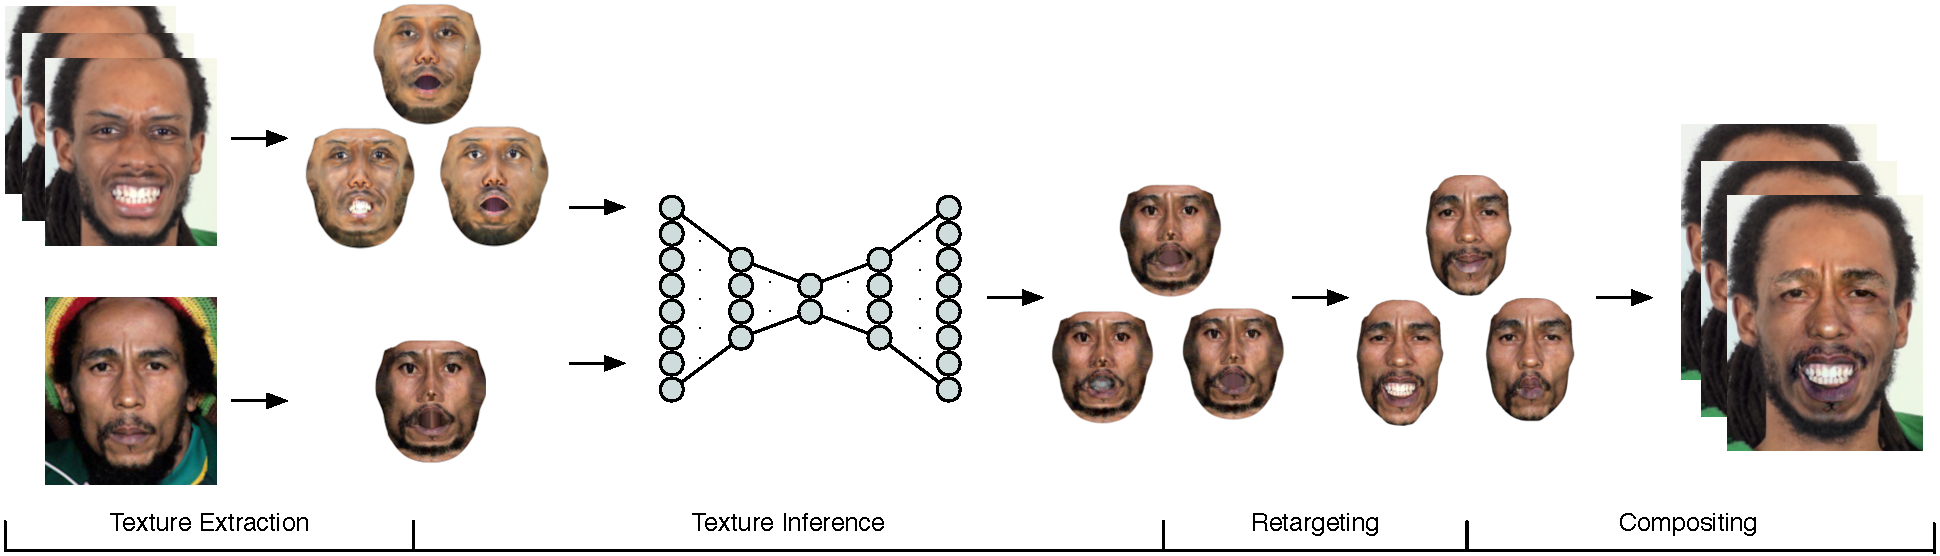
\includegraphics[width=1\linewidth]{figures/overview/overview.pdf}
	\caption{Overview of the pipeline.}\label{fig:arch_content}
	\vspace{-0.15in}
\end{figure*}


\subsection{Deep Generative Model for Texture Synthesis}

The rise of deep learning has brought many advances in image synthesis. Generative Adversarial Models \cite{gan} have proved especially capable of generating sharp and realistic images. 
More specifically, we use a conditional GAN~\cite{cgan} to enable end-to-end synthesis of high-resolution facial textures conditioned on the target identity and source facial expressions. While conditional GANs have been used for a wide range of applications such as image-to-image translation \cite{pix2pix}, face image generation \cite{gauthier2014}, image inpainting \cite{pathak2016context, yang2016high}, and style transfer \cite{li2016precomputed}, to our knowledge conditional generative adversarial models have never been used for the purpose of generating high-detailed textures.

Previous facial synthesis works that do not use conditional GANs include  \cite{liu2007face}, which hallucinates high-resolution faces from low-resolution images using a local patch-based Markov network, and
\cite{mohammed2009visio}, which generates novel face images by learning a probabilistic model from a set of training faces. 
However, neither of these results are realistic and artifact-free in high-resolution. \cite{golovinskiy2006statistical} uses statistical models to generate wrinkles and pores on facial geometry, but cannot do so for textures. \cite{saito2016} uses a deep learning framework to generate high resolution textures from a single image, but they cannot infer details like wrinkles and the inner mouth region on their textures for different expressions as we can.

\section{Overview}



%\subsection{Pipeline Overview}

%\subsection{The Joint Loss Function}


% Our pipeline is as follows (Fig.~\ref{fig:arch_content}):
Our pipeline consists of the following steps (illustrated in Fig.~\ref{fig:arch_content}):

\begin{enumerate}
\item Fit a 3D model to extract static albedo textures from each frame in the source video sequence and the single RGB target image (Section 4).
\item Infer dynamic textures and retarget the per-frame texture expressions from the source video frames onto the target image texture using a generative adversarial framework (Section 5).
\item Composite the target mesh with the generated dynamic textures into each frame in the source video (Section 6).
\end{enumerate}

% \vfill\eject

\section{Fitting the Face Model}


We model the face shape $S$ and albedo as a multilinear PCA model with $n = 53k$ vertices and $106k$ faces:
\begin{equation}
S(\beta_{id}, \beta_{exp}) = \hat{S} + B_{id}\beta_{id} + B_{exp} \beta_{exp}
\end{equation}
\begin{equation}
I(\alpha_{alb}) = \hat{I} + A_{alb} * \alpha_{alb}
\end{equation}
The identity and expression are represented as a multivariate normal distribution with $B_{id} \in \mathbf{R}^{3n \times 80} $, $B_{exp} \in \mathbf{R}^{3n \times 29}$ and $A_{alb} \in \mathbf{R}^{3n \times 80}$.  The dimensions of the mean shape are $\hat{S} = \hat{S}_{id} + \hat{S}_{exp} \in \mathbf{R}^{3n}$, and the mean albedo is given by $\hat{I} \in \mathbf{R}^{3n}$.  The standard deviations are given by: $\sigma_{id} \in \mathbf{R}^{80}$, $\sigma_{exp} \in \mathbf{R}^{29}$ and $\sigma_{alb} \in \mathbf{R}^{80}$.

We use the Basel Face Model ~\cite{blanz1999} for $B_{id}$, $A_{alb}$, $\hat{S}$ and $\hat{I}$ as well as FaceWarehouse ~\cite{cao2014facewarehouse} for $B_{exp}$. We model the illumination using second order Spherical Harmonics and assume Lambertian surface reflectance.  We denote the illumination as $L \in \mathbf{R}^{27}$.  

Following the optimization scheme of ~\cite{f2f}, we jointly solve for all the unknowns $\textbf{Y} = \{ S, I, R, t, P, L \}$ leveraging the Gauss-Newton method applied to iteratively re-weighted least squares with three levels of image pyramid, where P are the camera parameters. One can refer to ~\cite{f2f} for details of this optimization.  In short, our objective function is:
\begin{equation}
E(\textbf{Y}) = w_{col} E_{col}(\textbf{Y}) + w_{lan} E_{lan}(\textbf{Y}) + w_{reg}E_{reg}(\textbf{Y})
\end{equation}
We use energy weights $w_{col} = 1$, $w_{lan} = 10$ and $w_{reg} = 2.5 \times 10^{-5}$.  
The photo-consistency term is given by 
\begin{equation}
E_{col}(\textbf{Y}) = \frac{1}{| M | } \sum_{p \in M}  ||C_{gt}(p) - C_{render}(p)||_2
\end{equation}
 where $C_{gt}$ is the input image and $C_{render}$ is the synthesized image.  $p \in M$ denotes pixel visibility in the source image.  
The landmark term is given by: 
\begin{equation}
E_{lan}(\textbf{Y}) = \frac{1}{|F|} \sum_{f_i \in F}  || f_i - \Pi_P(RS_i + t) ||_2^2
\end{equation}
 where $f_i \in F$ is a 2D facial feature following the method presented in ~\cite{kazemi2014one}.  
The regularization $E_{reg}$ term ensures that faces stay close to the normal distribution.  This term prevents degenerative faces when performing the fitting:
\begin{equation}
E_{reg}(\textbf{Y}) = \sum_{i = 1}^{80} [ (\frac{\beta_{id, i}}{\sigma_{id,i}})^2 + (\frac{\alpha_{alb, i}}{\sigma_{alb, i}})^2] + \sum_{i =1}^{29} ( \frac{\beta_{exp,i}}{\sigma_{exp,i}})^2
\end{equation}

\section{ Dynamic Texture Synthesis}

\subsection{Deep Learning Framework}

\begin{figure*}[th]
	\centering
	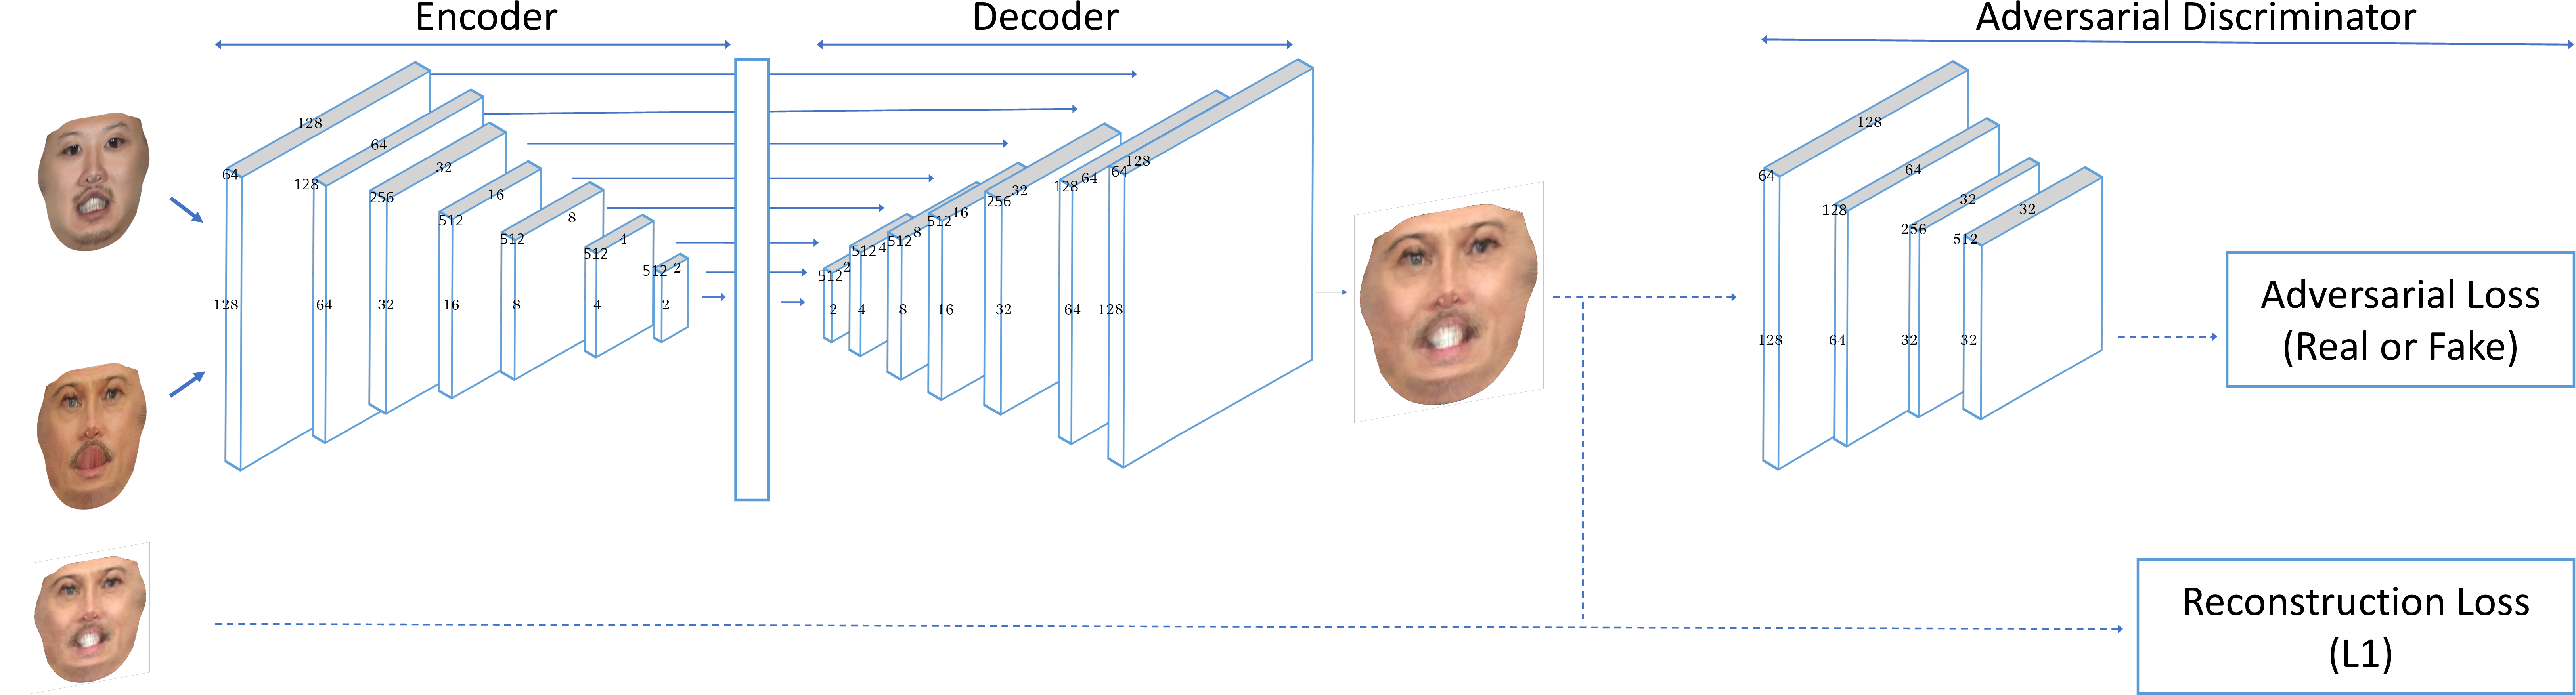
\includegraphics[width=1\linewidth]{figures/network/network.png}
	\caption{The network architecture. The encoder takes as input the identity texture and the expression texture, and the decoder outputs the dynamic texture. The adversarial discriminator is used during training to judge whether the output texture looks real or not.}\label{fig:network}
	\vspace{-0.15in}
\end{figure*}

The core of our dynamic texture synthesis pipeline for inferring fine details is a Conditional Generative Adversarial Network used to infer deformations from a source texture onto a target texture.
Broadly speaking, a Generative Adversarial Network (GAN) $G$ is a function which produces ``realistic'' output from a noise vector.  
That is, given a distribution $M$, a variable $z \sim M$, and a set of ground truth ``real'' examples $X$,  we would like $G(z)$ to be indistinguishable between 
any $x \sim X$.  Formally, by indistinguishable we mean to say that the generator function fools as best as possible a discriminator function, $D$, 
trained precisely to separate the generated output $G(z)$ from the real output drawn from $X$. A conditional GAN, on the other hand, takes as input both the noise vector $z$, along with additional input $y$ in order to produce the output $x$.    
Notice that $y$ and $x$ are not necessarily from the same set.  

In our setting, we attempt to learn a target texture deformation given a source texture deformation.  
That is, given a source texture $U_{source}$ that encodes a given expression, we would like to transfer this expression to a neutral-pose target texture $N_{target}$.  
For example, the source texture expression might contain a wrinkle on the left cheek that we would like to synthesize onto the target neutral texture. 
In this case, the output is $U_{target}$, the target texture with the wrinkle, and we are conditioning on $U_{source}$ and $N_{target}$.  


Note that neural networks are inclined to be heavily affected by noise and variation within the training corpus.  For this reason, we work in the UV texture space of the captured facial albedos.  This provides many benefits during training.  First of all, it minimizes variations in the input due to factors such as lighting, image background and head pose. In UV space, the mouth, eyes, and nose are in the exact same location in each image - the only thing that changes is the content of those locations. Working in this space makes it possible to retarget mouth motion, blinking, scrunching, and various other skin deformations that would be much harder to learn otherwise.  


\subsection{Loss Function}

The energy function we minimize is given by 
\begin{equation} \label{eqn:1}
\begin{split}
L_{GAN}(G,D)& = E_{{x,y}\sim p_{data}({x,y}),z\sim p_z{z}}[\log D({t})]\\
& +E_{{x,y}\sim p_{data}(x),z\sim p_z(z)}[\log(1-D(G(x,z)))] 
\end{split}
\end{equation}

In our formulation, $x$ is the pair $(U_{source}, N_{target})$ and $y$ is given by $U_{target}$.  
In addition to this energy, the generator $G$ also attempts to minimize the reconstruction loss to the target $y$ in the L1 sense.  
That is, $L_{recon}(G)= E[\parallel y-G({x,y},z)\parallel_1]$ ~\cite{pix2pix}.

$G$ attempts to minimize this objective while $D$ attempts to maximize it.  In other words:
$ G_{opt}=\text{arg}\min\max L_{cGAN}(G,D)+\lambda L_{L1}(G)$, where $\mu$ 
encodes the relative weighting of the different errors ~\cite{pix2pix}.  In our implementation of the conditional GAN, 
we do not input any noise during generation, but otherwise the optimization program is accurate.  We set $\mu = 0.001$ in all experiments. 
This parameter can be viewed as a balancing between the need to reconstruct accurate wrinkles with the need to have the final texture
remain "realistic".  

\subsection{Network Architecture}


We use a similar architecture as \cite{pix2pix}. 
First, we concatenate the driver expression and the neutral target identity, $(U_{source}, N_{target})$, along their color-channel dimension as input.
The generator output is the target expression $y$, which is the expression transferred from the source to target texture.

Second, we use a masked prior to define the $\ell_1$ and adversarial loss. 
The mask is applied on the $\ell_1$ loss such that the the loss around the mouth and eye regions is ten times higher than in other areas - we
do this because wrinkles, blinking, and most texture deformations are a lot more prevalent in these areas.  
For the discriminator, we adopt a Markovian Discriminator 
(PatchGAN) with patch size set to $70 \times 70$. We found that adding skip connections between
encoder layers and decoder layers, skipping around the code layer, greatly reduces noise in the output image. 
%Finally, we do not input any 
The parameters are
optimized using ADAM with back-propagation. Our input and output resolution are $256\times 256$.


%%\begin{eqnarray*}
%%G^*&=&arg\min\max L_{cGAN}(G,D)+\lambda L_{L1}(G) \\
%%L_{L1}(G)&=& E[M\cdot\parallel y-G({x,y},z)\parallel_1] \\
%%L_{GAN}(G,D)&=& E_{{x,y}\sim p_{data}({x,y}),z\sim p_z{z}}[\log D({t})]+E_{{x,y}\sim p_{data}(x),z\sim p_z(z)}[\log(1-D(G(x,z)))]
%%\label{eqn:1}
%%\end{eqnarray*}

\subsection{Mouth Synthesis}

\begin{figure}[h]
	\centering
	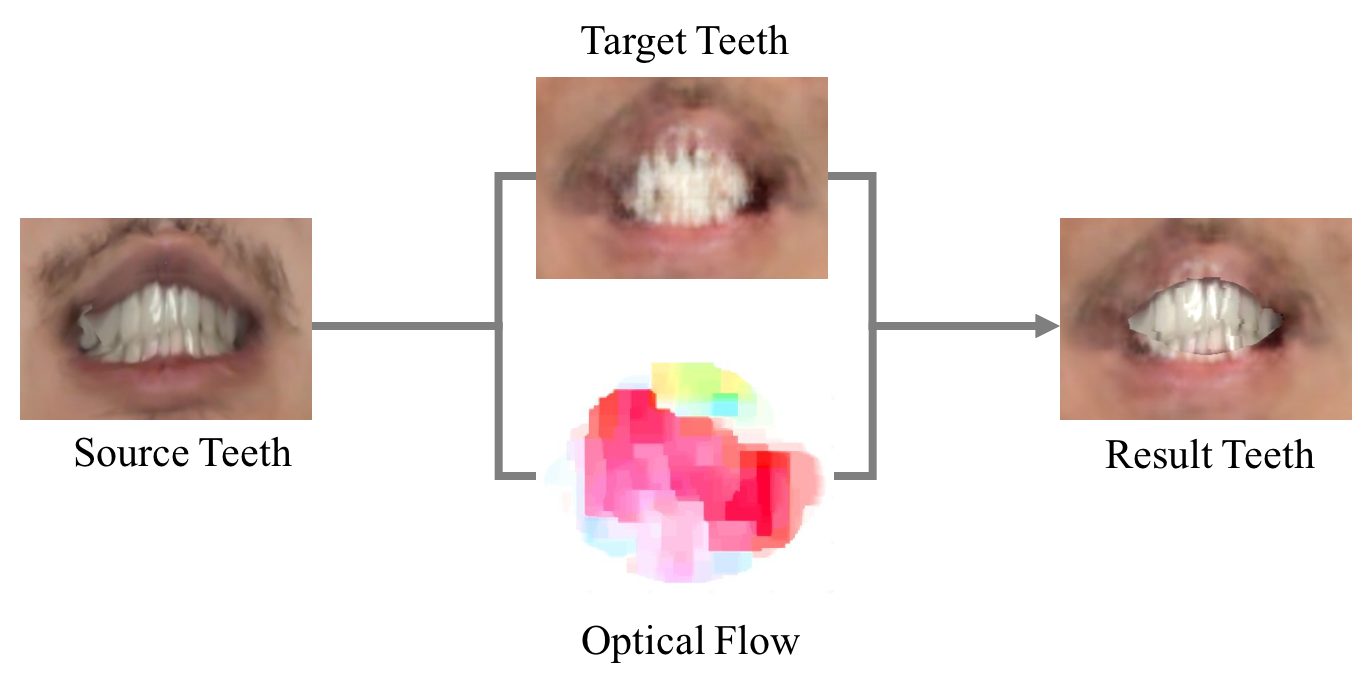
\includegraphics[width=1\linewidth]{figures/flow/opticalflow2.png}
	\caption{Visualization of flow-upsampling from source mouth to low-resolution inferred mouth.  Left is source mouth, top is target mouth, bottom is flow field, right is final result.}\label{fig:flow}
	\vspace{-0.05in}
\end{figure}
We model the mouth interior region as a part of the UV texture.  When the mouth is closed, the area between the lips get projected onto this area to
make a pink color.  When the mouth is open, the mouth interior, including the teeth and tongue, are projected to this region (Fig.~\ref{fig:flow}).  

Using our deep-learning framework, we are able to transfer open-mouth expressions onto the closed-mouth neutral target textures and infer the
inner mouth region.  However, due to lack of training data for the mouth interior, the inferred texture here tends to be of rather low resolution.  In order
to improve this area, we use SIFT-Flow ~\cite{siftflow} to redraw the target mouth using the source mouth for each frame.  In particular, after
computing SIFT features at the pixel level, we perform matching based on the following energy term:
\begin{equation}
\begin{split}
E(w)& = \sum_p \min (||s_1(p) − s_2(p + w(p))||_1, t)  \\
&\hspace{-6mm} +\sum \eta(|u(p)| + |v(p)|)  \\
&\hspace{-6mm} +\sum_{(p,q) \in \epsilon} min(\alpha |u(p) - u(q)|, d) + min(\alpha|v(p) - v(q)|, d)
\end{split}
\end{equation}
The terms in the equation are, in order, the data term, the small displacement term, and the spatial regularization term ~\cite{sift}, 
where $w(p) = (u(p), v(p))$ is the flow vector at a point $p = (x,y)$, and $s_1$ and $s_2$ are the sift features
compunted for either image 1 or image 2 at the point $p$.  The second and third term regularize the matching by pushing
nearby points to get mapped to each other.

Inferring the inner mouth also has the added benefit of improving the lip texture around the mouth during tracking failure of the original video: tracking of tight-lipped
expressions such as kissing often fail and the lip texture gets projected to the interior region in UV space.  During rendering, this causes
the lips to be thinner than they should be, which gives an unnatural appearance.  By inferring this inner-mouth region, we are able to synthesize realistic 
kissing faces on the target even when lip tracking fails on the source.

%\subsection{Fitting to Video Sequence}

%We adopt a similar optimization scheme as ~\cite{f2f} to obtain the per-frame mesh and per-frame texture of the source video sequence at run-time.  In particular:

%%IMPLEMENTATION DETAILS OF F2F

%Using the per-frame texture, we synthesize per-frame textures and mouth flows using the above framework on the single RGB target image, and then
%are able render a realistic animation of the target.  

\section{Video Face Replacement via Blending}

Once we have the per-frame textures and retargeted mesh, we are also able to transfer the target appearance back onto the source video
sequence for a detailed and realistic animation (Fig.~\ref{fig:blend}). We use a graph-cut approach similar to ~\cite{replace} in order 
to achieve this.  In particular, for blending the retargeted faces to the source video in a photorealistic manner,
we first find a graph-cut to partition each frame into two regions, which determines whether 
a pixel comes from the frame in the source video or the image of the rendered retargeted face model(Fig.~\ref{fig:blend}a-c). 
We then linearly blend the target and source regions of the images along the seam to achieve a smooth and realistic result (Fig.~\ref{fig:blend}d).
 
\begin{figure}[t]
  \centering
  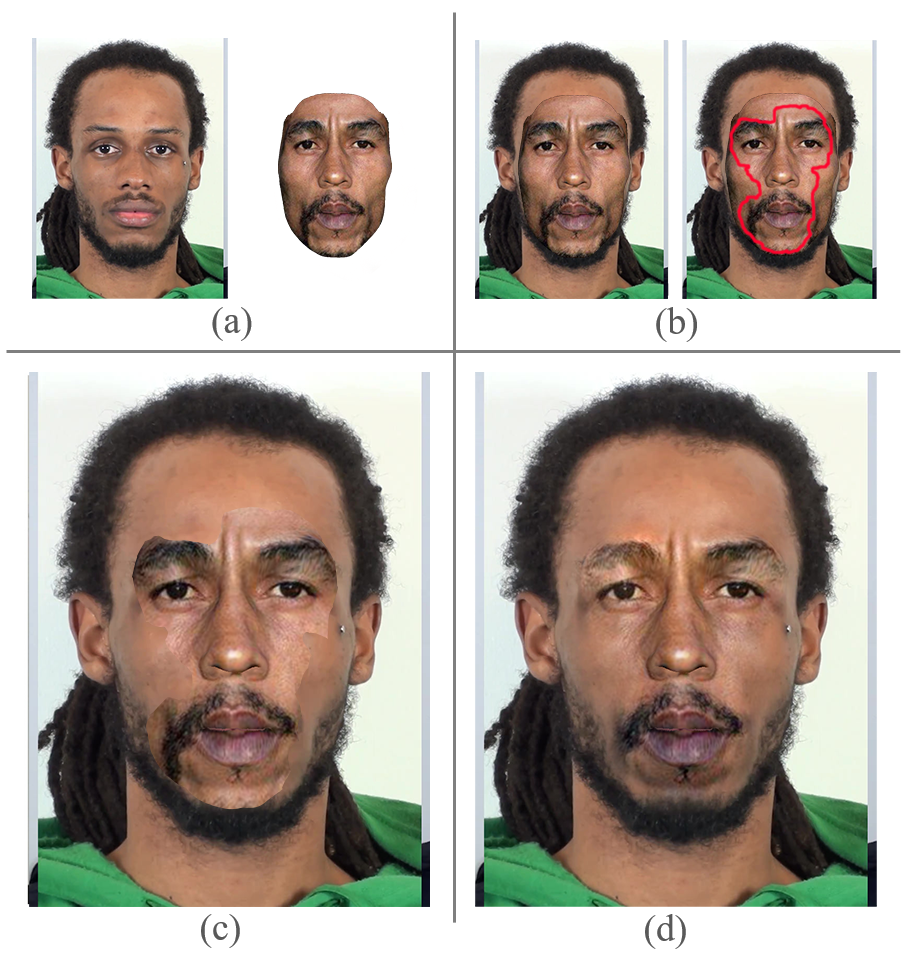
\includegraphics[width=0.6\linewidth]{figures/blending/blending_new_tidus.png}
  \caption{a) The input consists of the frames of the source video (left) and the rendered retargeted mesh (right). b) Naively projecting all of the target mesh's vertices onto the source frame results in an unrealistic and incoherent result (left) when a more optimal partition is outlined in red on the image on the right. 
	c) The composition of the two images using the optimal scene.
	d) Linearly blending the pixels along the seam gives a smooth and realistic result.}
	\label{fig:blend}
  \vspace{-0.15in}
\end{figure}



\subsection{Graph-Cut}
Similar to ~\cite{replace}, 
we optimize the partition so as to ensure spatial coherence coherence between neighboring pixel values
and temporal coherence between frames. 


If we naively project the mesh back onto the frame of the source video, as seen in the left-hand image of Fig~\ref{fig:blend}b, the result is not smooth or realistic. 
In order to maintain spatial coherence across large variations in pose and expression, 
 we construct a graph-cut problem on each of the frames in the source video and their corresponding retargeted mesh as in ~\cite{graphcut}. For each frame, the graph cut algorithm labels each vertex on the mesh as either a source vertex or target vertex in a manner that minimizes the difference in pixel values across neighboring vertices, as shown on the right-hand image of Fig.~\ref{fig:blend}b. We then project the seam of the labeled mesh onto the image (Fig.~\ref{fig:blend}c). 

The nodes of the graph represent the vertices on the mesh for each frame in the source video. 
Let each vertex be denoted as $V_{t,i}$, where $t$ refers to the $t$th frame, and $i$ refers to the $i$th vertex on the mesh. 
%and construct the following graph to calculate the seam in the rest region.

In order to minimize the difference between source and target pixels along the seam, for each frame, we set weights on the graph for each edge between each pair of vertices $V_{t,u}$ and  $V_{t,v}$ that share an edge on the mesh as:
\begin{equation}
\begin{split}
W_m(V_{t,u}, V_{t,v}) = & \|I_{s}(V_{t,u})-I_{s}(V_{t,v})\|\\
& + \|I_{t}(V_{t,u})-I_{t}(V_{t, v})\| 
\end{split}
\end{equation}

 $I_{s}$is the source image, $I_{w}$ is the target image, $I_{s}(V)$ is the color at the pixel where $V$ is projected onto the source frame, and $I_{t}(V)$ is the color at the pixel V is projected onto in the rendered target image.
 For temporal coherence, we set edges between vertices $V_{t,i}$ and $V_{t+1,i}$ for all $i$ and $t$, with weight as:
\begin{equation}
\begin{split}
W_f(V_{t,i}, V_{t+1,i})& = \lambda \|I_{s}(V_{t,i})-I_{s}(V_{t+1,i} +1)\|^{-1}\\
              & + \|I_{t}(V_{t,i})-I_{t}(V_{t+1,i} + 1)\|^{-1}
\end{split}
\end{equation}

After computing the seam, we can composite the target appearance onto the source video and linearly blend the pixels across the seam for a realistic novel reenactment.  







\section{Experiments}

\subsection{Data Collection}

In order to semantically transfer similar expressions from one texture to another, the training data must be collected in a way so that 
corresponding expression textures across different individuals are aligned.  To do this, we hired actors to perform a series of 21 expressions based on the Facial Action Coding System (FACS) ~\cite{Ekman:1978}, and recite 20 Harvard Sentences ~\cite{HarvardSent:1969}. We then hand cut, warped, and aligned the sequences using video editors.  Each FACS expression was broken
up and extended into two 24-frame sequences.  The first of these consisted of an individual starting on neutral frame, then moving to the apex of the FACS expression.
The second 24-frame sequence was a different clip of the face starting in the FACS expression and returning to neutral.  The sentences were aligned
using dynamic time warping on the audio sequences to align the video sequences, as was done in ~\cite{olszewski2016high}. We plan to release this synchronized, high-resolution dataset to the public in the future. 

After aligning the sequences, we used a face-tracking and texture extraction process based on the formulation of ~\cite{f2f}, to compute a texture
for each of the aligned video frames. Our total dataset consists of a set of 15 identities, each with 3107 frames. We use 12 of these for training our network and withhold 3 for validation. We also captured additional subjects used for generating the final results and performing quantitative evaluation (see Results below).

\subsection{Data Augmentation}
In order to increase the generalization ability of our network to subjects whose appearance varies significantly from those in this dataset, we augment it by altering the skin tones of the captured textures. Specifically, we extract lighting-independent and expression-free albedos from the texture images.
We then perform PCA on the albedo images. To each albedo image, we add multiples of the found principal components with magnitudes proportional to the corresponding eigenvalues multiplied with a random variable drawn from a Gaussian with mean zero and standard deviation 0.1. This results in a new series of albedo images that differ from the original in their skin tone and local details.

These albedo textures, combined with the unmodified captured albedo textures, are used as the training data for our network. We generate 15 additional albedo textures from each subject, giving us a total of 559,260 training images from the 12 training subjects.

\subsection{Training and Testing}

We divide the dataset into a training set and a testing set. During training, we train the network in an end-to-end fashion. On each iteration, we randomly sample a pair consisting of a source expression frame and a target identity frame from the dataset as input. The corresponding ground truth texture combining the given identity and expression is also sampled. The output will be synthesized using a forward pass, and the loss is back-propagated using Adaptive Moment Estimation (ADAM). The images are scaled to $256 \times 256$ and we set each batch to contain 64 images. We trained the networks on a Titan X GPU until both the generative loss and discriminative loss converged, which took roughly two days (the training and validation loss diagrams can be found in the supplementary material). We set the initial learning rate to $lr=2\mathrm{e}{-4}$ for the generator and $lr=2\mathrm{e}{-5}$ for the discriminator. The learning rate is lowered several times during training. During testing, we randomly sample a pair consisting of a source expression frame and a target identity frame from the test set.

\section{Results}

As input our system takes a source video and a single target image of a face. It generates a dynamic texture of the target image for a 3D model and retargets the source mesh onto the single input image, inferring details such as wrinkles and the inner mouth region.  Our results can be seen in Fig.~\ref{fig:result}. More results can be seen in the supplementary material.


\paragraph{Reenactment: Comparison To Previous Works}

When given only a single image as a target input, \cite{f2f} can only generate static textures and does not capture any of the wrinkles or inner mouth details that our system captures as seen in Fig.~\ref{fig:result}. 

An example of methods like \cite{f2f} that do not use our inference model, thereby producing less detailed results when there is only a single target image as input, can be seen in Fig.~\ref{fig:wrinkles}.


\begin{figure}[th]
	\centering
	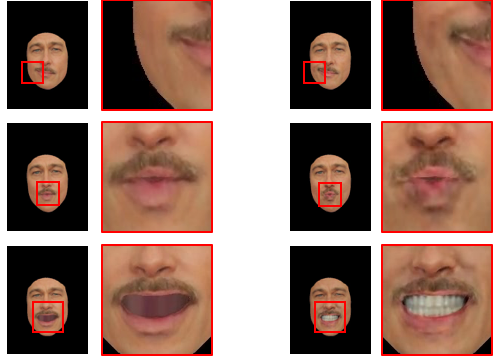
\includegraphics[width=1.0\linewidth]{figures/wrinkles/example_crop.png}
	\caption{Wrinkle animations from a single neutral target input image. In each row, the pair of images on the left shows the facial animation achieved using a static texture generated by a classical correspondence methods such as Face2Face. The pair of images on the right show the facial animation achieved using the dynamic texture generated by our inference model. Note that the images on the right are capable of generating detailed wrinkles and filling the inner mouth cavity.}~\label{fig:wrinkles}
	\vspace{-0.2in}
\end{figure}
\paragraph{Composition: Comparison To Previous Works}

\cite{replace} is currently the state-of-the-art with respect to face composition, and their results are shown in Fig.~\ref{replaceres}. Our results for composition in Fig.~\ref{fig:result} are comparable to theirs, but we only need a single target image as input while they need a video sequence.

\begin{figure}[th]
\begin{center}
   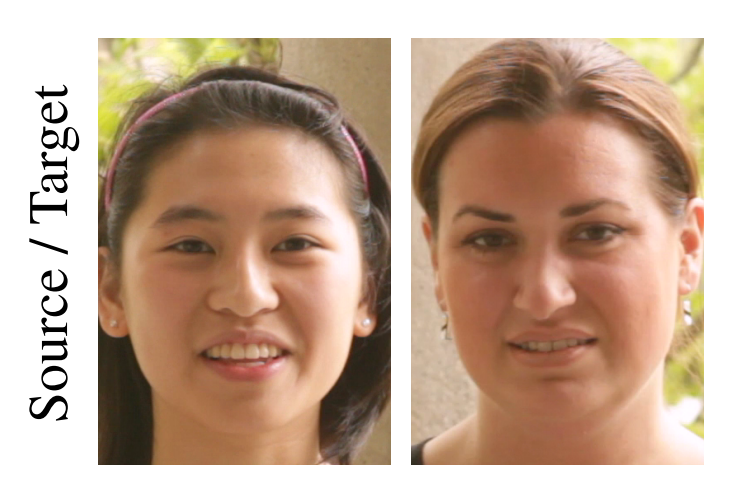
\includegraphics[height=90px]{figures/results/daleaa.png}
   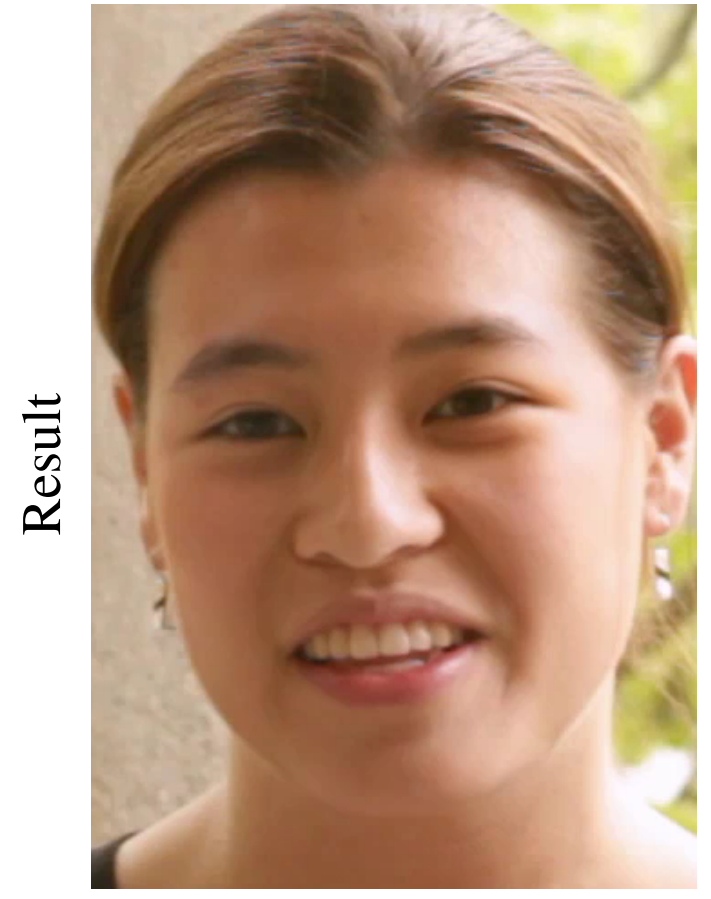
\includegraphics[height=88px]{figures/results/dalebb.png}
\end{center}
   \caption{\protect\cite{replace} takes two video inputs and can do face replacement as shown in this figure. Our results are comparable to the results in this figure, but we are only using a single target image as input. Furthermore, \protect\cite{replace} cannot handle only a single target image as input.}
   \vspace{-0.05in}
\label{replaceres}
\end{figure}

% TODO: reference to the table. The caption should be fleshed out.
\begin{figure}[th]
\begin{center}
  
\includegraphics[width=0.24\columnwidth]{figures/kylehao_transfer/raw000762.png}
   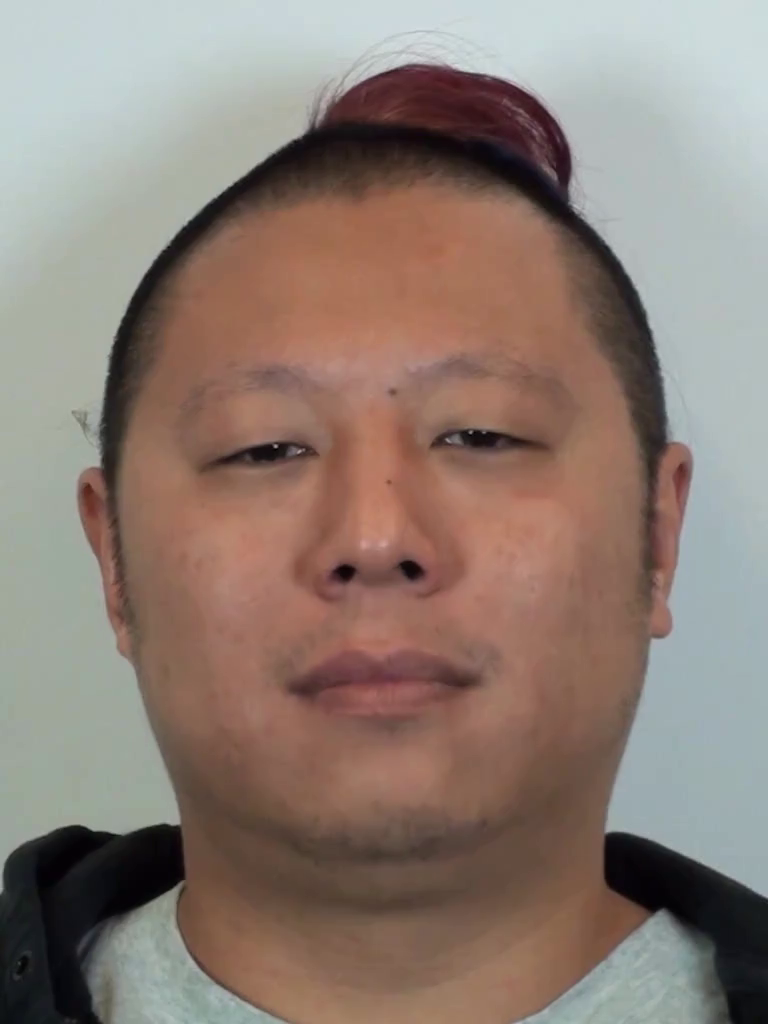
\includegraphics[width=0.24\columnwidth]{figures/kylehao_transfer/raw000001.png}
   
\includegraphics[width=0.24\columnwidth]{figures/kylehao_transfer/static_000762.png}
   
\includegraphics[width=0.24\columnwidth]{figures/kylehao_transfer/dynamic_000762.png} 
\end{center}
   \caption{Non-frontal face reenactment. From left to right: the source image, the target image, the static texture and the dynamic texture. We can see that the dynamic texture contains more details like the wrinkles.}
   \vspace{-0.05in}
\label{replaceres}
\end{figure}

% TODO: reference to the table. Did we take average over all the images? The names of the
% methods in the table should be fleshed out. The caption should be fleshed out.
\begin{table}[h!]
\begin{center}
\resizebox{.45\textwidth}{!}{%
  \begin{tabular}{ l  c  c c}
    \hline
    Method & Mean L1 Loss & Mean L2 Loss & SSIM \\ \hline
    \emph{transf} & 1360 &  152 & 0.8730 dB\\ \hline
    \emph{diff} & 1790  & 211 & 0.8150 dB\\ \hline
\end{tabular}}
\end{center}
\caption{Numerical comparison.}
\vspace{-0.2in}
\label{table:paris}
\end{table}


\setlength{\tabcolsep}{3pt}
\begin{figure*}[th]
	\centering
	\includegraphics[width=.93\linewidth]{figures/results/figure6.pdf}
	\vspace{0.4cm}
	\caption{Two sample results of our method. Top row of each example shows the source video sequence. Middle row shows the target single-frame input and the animated retargeted faces. Bottom row shows the compositing result.}
    \label{fig:result}
\end{figure*}


% \vfill\eject

\section{Discussion}

We present a method of generating realistic video sequences of faces from a single photograph 
which can then be used to replace the face of a source/driver video sequence. 
To the best of our knowledge, our method is the first
to leverage GANs to produce realistic, high-resolution dynamic textures from a single target input image to be used for rendering.  

\paragraph{Limitations and Future Work}
Though we are able to infer dynamic textures, the input target face is assumed to be without extreme specular lighting and/or pronounced shadowing. If present, thse can cause the texture extraction phase following ~\cite{f2f} to produce artifacts. As fitting the facial geometry precisely from a single viewpoint is a highly underconstrained problem, the extracted texture of the target subject may be improperly registered in extreme cases in which this fitting is insufficiently accurate. Other issues resulting from imperfect fitting include missing transient expressions, such as blinking. We believe that it is possible to address these issues with a more robust multilinear fitting, which takes greater account of specular lighting, shadowing, shading, and variation in the subject's appearance.   

The resolution of the single image of the target must be sufficiently high resolution in order to generate appropriate details for the corresponding expressions. Furthermore, as we rely on the method of~\cite{f2f} to extract both the source and target textures, if either is largely non-frontal/occluded, the textures will be incomplete which causes artifacts in the synthesis.  Our method produces reasonable results in the non-occluded regions, but cannot synthesize unseen parts. However, this problem can be addressed by applying the method of ~\cite{saito2016} to infer the invisible face regions before completing the detail transfer.  For these reasons, compositing for non-frontal views will not be as realistic.  We have additional non-frontal synthesis and retargeting results in the supplementary materials.  


Limited variation of appearance in the training corpus is also an issue.  Though the data augmentation mitigates this, the generated wrinkles and deformations will not be as sharp or as strong when the target's appearance varies greatly from those in our dataset.  However, we believe that having a larger dataset with even greater appearance variations would resolve this issue. Finally, we note that the method solves for each frame of animation independently, and so can potentially result in temporal incoherency, e.g. flickering.  We can accomodate for this in future work by solving for multiple frames simultaneously, or by applying temporal smoothing in a post-processing step.  

\vfill\eject



{\small
\bibliographystyle{ieee}
\bibliography{iccv}
}

\end{document}
